\documentclass{BeamerTemplate}
\title{Module 3 - Quelques lois de probabilité discrètes}
\subtitle{STT-1000 Probabilités et statistique}
\date{\today}

% Lien discret vers la page de réponses, ajouté au pied de page à côté du numéro
% (ne prend aucune place sur la diapo). Usage, n'importe où dans la diapo : \lienreponse{rep-ex}
\newcommand{\cibleReponse}{}
\newcommand{\lienreponse}[1]{\gdef\cibleReponse{#1}}
\addtobeamertemplate{footline}{}{%
  \ifx\cibleReponse\empty\else
    \begin{tikzpicture}[remember picture,overlay]
      \node[anchor=south east, inner sep=0pt] at ([xshift=-1.5cm,yshift=0.2cm]current page.south east)
        {\hyperlink{\cibleReponse}{\scriptsize\color{gray}Réponse~$\rightarrow$}};
    \end{tikzpicture}%
    \global\let\cibleReponse\empty
  \fi}
% Lien de retour vers l'exemple, dans les pages de réponses
\newcommand{\retour}[2]{\hyperlink{#1}{\textbf{#2}~{\color{gray}$\hookleftarrow$}}}

% Graphiques des fonctions de probabilité (valeurs exactes calculées d'avance)
\pgfplotsset{
  loi/.style={
    width=6.1cm, height=3.95cm, axis lines=left, ymin=0, enlarge x limits=0.03,
    tick label style={font=\tiny}, label style={font=\scriptsize},
    xlabel={$x$}, ylabel={$p(x)$}, ylabel style={yshift=-2pt},
    scaled y ticks=false,
    yticklabel style={/pgf/number format/.cd, fixed, fixed zerofill, precision=2, use comma},
  },
  baton/.style={ycomb, thick, black, mark=*, mark size=0.9pt},
}

\begin{document}

\begin{frame}
\titlepage
\end{frame}

\section{Introduction}

\begin{frame}{Contexte}

Plusieurs lois discrètes sont si fréquentes qu'elles portent un nom; on connaît bien leur comportement et leurs caractéristiques.

\vspace{0.2in}
Plusieurs de ces lois découlent d'expériences aléatoires simples, par exemple une expérience qui se solde par un succès ou un échec. \\
Ex. : on lance une pièce de monnaie; on déclare un succès si on obtient pile et un échec si on obtient face.

\vspace{0.2in}
Nous verrons cinq de ces lois dans le cours.

\end{frame}


\begin{frame}[t]{Quelques résultats utiles pour les preuves}

\begin{itemize}
 \item {\bf Théorème du binôme (rappel) :}
 $$\sum\limits_{i=0}^n{n\choose i}x^iy^{n-i}= (x+y)^n$$
 \item {\bf Séries géométriques :}
 $$ \sum_{i=0}^n p^i = \frac{1-p^{n+1}}{1-p}$$
 $$ \sum_{i=0}^{\infty} p^i = 1+p+p^2+\cdots=\frac{1}{1-p} \; \; \; \alerter{ \mbox{ si } |p|<1}$$
  \item {\bf Développement de $e^x$ :} $$e^x=1+x+\frac{x^2}{2!}+\frac{x^3}{3!}+\cdots=\sum\limits_{i=0}^\infty\frac{x^i}{i!}$$
\end{itemize}
\end{frame}


\begin{frame}[t]{Un concept important : v.a. indépendantes}

{\small
Il sera question à quelques reprises de \alerter{variables aléatoires indépendantes}, un concept défini formellement plus tard. Pour l'instant :
\alerter{deux variables aléatoires sont indépendantes si connaître la valeur de l'une ne nous apprend rien sur la valeur de l'autre.}
On note alors $X \perp Y$.

\smallskip
Deux propriétés utiles :
\begin{itemize}
\item $E(X_1+\cdots+X_n)=E(X_1)+\cdots+E(X_n)$, \alerter{toujours};
\item $V(X_1+\cdots+X_n)=V(X_1)+\cdots+V(X_n)$ si les $X_i$ sont \alerter{indépendantes}.
\end{itemize}
}

\begin{Boite}{Exemple}
{\footnotesize
Je lance un dé et une pièce de monnaie. Soit $X$ le résultat du dé, et $Y=0$ si la pièce tombe sur pile, $Y=1$ si elle tombe sur face. $X$ et $Y$ sont indépendantes : le résultat du dé n'a aucune influence sur celui de la pièce, et inversement.
}
\end{Boite}

\end{frame}

\section{Loi de Bernoulli}

\begin{frame}[t]{Loi de Bernoulli}
Soit $X$ une variable aléatoire telle que $X=1$ si l'expérience est un succès et $X=0$ si c'est un échec. On associe une probabilité $p$ au succès et $1-p$ à l'échec.

\bigskip
On dit que $X$ suit une loi de Bernoulli de paramètre $p$, ce qu'on note
$$X\sim \mbox{Bernoulli}(p).$$

La fonction de probabilité de la loi de Bernoulli$(p)$ est
$$
p(x)=\left\{\begin{array}{ll}
p, & x=1\\
1-p, & x=0\\
0, & \text{sinon.}
\end{array}\right.
$$

\end{frame}

\begin{frame}[t]{Loi de Bernoulli : espérance et variance}

\textbf{Espérance} :

\vspace{2cm}

\textbf{Variance} :

\end{frame}

\section{Loi binomiale}

\begin{frame}[t]{Loi binomiale : définition}
Soient $Y_1,\ldots,Y_n$ des variables aléatoires indépendantes de même loi de Bernoulli, c'est-à-dire $Y_i\sim \text{Bernoulli}(p)$ pour tout $i = 1,\ldots,n$.

\medskip

Soit $X$ le nombre total de succès parmi $Y_1,\ldots,Y_n$ :
$$X=\sum_{i=1}^nY_i.$$

\medskip
On dit que $X$ suit une loi binomiale de paramètres $n$ et $p$, ce qu'on note
$$X\sim \mbox{Binomiale}(n,p).$$
\end{frame}

\begin{frame}{Loi binomiale : fonction de probabilité}

{\small

On cherche $p(x) = P(X = x) = P(\mbox{observer $x$ succès}).$

\vspace{0.1 in}
On veut $x$ succès, donc $n-x$ échecs. Puisque les essais sont indépendants, chaque suite de résultats comptant $x$ succès et $n-x$ échecs a une probabilité de

$$ p^x (1-p)^{n-x}.$$

Il faut tenir compte du nombre de façons de placer les $x$ succès parmi les $n$ essais :

$$\displaystyle \binom{n}{x}.$$

Donc, si $X\sim \text{Binomiale}(n,p)$, alors
$$p(x)=\left\{\begin{array}{ll}
{n\choose x}p^x(1-p)^{n-x}, & x=0,1,\ldots,n,\\
0, & \text{sinon}.
\end{array}\right.$$

}

\end{frame}


\begin{frame}{Loi binomiale : vérification}

Vérifiez que la fonction $p(x)$ ci-dessus est bien une fonction de probabilité.

\end{frame}


\begin{frame}{Loi binomiale : allure}

\begin{center}
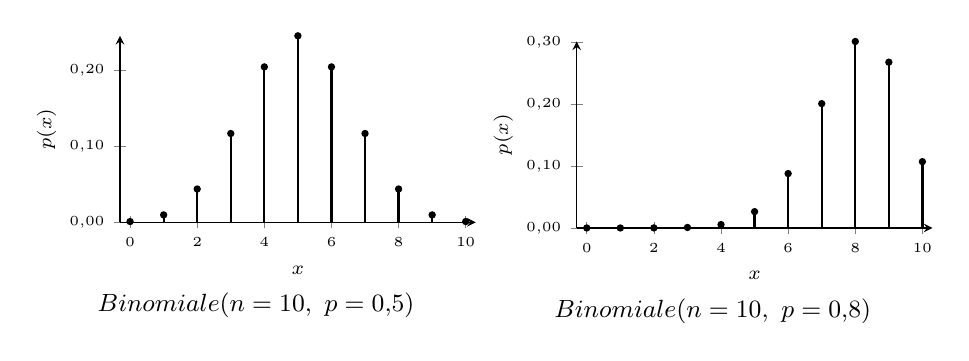
\begin{tikzpicture}
\begin{axis}[loi, xtick={0,2,...,10}, name=g]
  \addplot[baton] coordinates {(0,0.00098) (1,0.00977) (2,0.04395) (3,0.11719) (4,0.20508) (5,0.24609) (6,0.20508) (7,0.11719) (8,0.04395) (9,0.00977) (10,0.00098)};
\end{axis}
\node[anchor=north, font=\small] at (g.outer south) {$\text{Binomiale}(n=10,\ p=0{,}5)$};
\begin{axis}[loi, xtick={0,2,...,10}, name=d, at={([xshift=0.9cm]g.outer east)}, anchor=outer west]
  \addplot[baton] coordinates {(0,0.00000) (1,0.00000) (2,0.00007) (3,0.00079) (4,0.00551) (5,0.02642) (6,0.08808) (7,0.20133) (8,0.30199) (9,0.26844) (10,0.10737)};
\end{axis}
\node[anchor=north, font=\small] at (d.outer south) {$\text{Binomiale}(n=10,\ p=0{,}8)$};
\end{tikzpicture}
\end{center}

\medskip
{\small
Dans tous les cas :
\begin{itemize}
\item les valeurs possibles sont $0,1,2,\ldots,n$;
\item la valeur la plus probable est proche de $np$ (c'est la partie entière de $(n+1)p$);
\item la fonction de probabilité croît jusqu'à cette valeur, puis décroît.
\end{itemize}
}

\end{frame}

\begin{frame}[t]{Loi binomiale : espérance}
Si $X\sim \text{Binomiale}(n,p)$, alors $E(X)=np$.

\smallskip
Plus simplement : $X=Y_1+\cdots+Y_n$, donc $E(X)=$

\vspace{0.9cm}
{\footnotesize
Preuve directe :
\vspace{-2mm}
\begin{align*}
E(X) = \sum_x x\, p(x) &= \sum_{x=0}^{n} x {n\choose x}p^x(1-p)^{n-x}
= \sum_{x={\color{red}1}}^{n} x \frac{n!}{x!(n-x)!}p^x(1-p)^{n-x} \\
&= np \sum_{x=1}^{n} \frac{(n-1)!}{(x-1)!(n-x)!}p^{x-1}(1-p)^{n-x} \\
&= np \sum_{y=0}^{n-1} \frac{(n-1)!}{y!(n-1-y)!}p^{y}(1-p)^{n-1-y} \quad \mbox{(en posant } y=x-1\mbox{)}\\
& = np
\end{align*}
\vspace{-2mm}
{\color{gray} D'où vient la simplification qui permet de passer de l'avant-dernière ligne à la dernière?}
}

\end{frame}

\begin{frame}[t]{Loi binomiale : variance}

{\small

On peut calculer $V(X)$ de la même façon que $E(X)$.

\smallskip
Plus simplement : \alerter{si $X \sim \text{Binomiale}(n,p)$, on peut écrire $X = Y_1 + \cdots + Y_n$, où les $Y_i$ sont des variables aléatoires indépendantes de loi Bernoulli$(p)$.}

\begin{align*}
V(X) &= V\left(\sum_{i=1}^n Y_i \right)\\
&= \sum_{i=1}^n V(Y_i) \; \; \mbox{ car } Y_i \perp Y_j, \ i \ne j \\
&= \sum_{i=1}^n p(1-p) \; \; \mbox{ car } Y_i \sim \mbox{Bernoulli}(p), \ \forall i\\
&= np(1-p)
\end{align*}

}

\end{frame}

\section{Loi géométrique}

\begin{frame}[t]{Loi géométrique : définition}
On suppose
\begin{itemize}
 \item une suite d'essais \alerter{indépendants};
 \item chaque essai se solde par un succès ou un échec;
 \item la probabilité de succès \alerter{à chaque essai} est $p$;
 \item on arrête l'expérience dès qu'on obtient \alerter{un premier succès}.
\end{itemize}

\medskip
Soit $X$ le \alerter{nombre total d'essais nécessaires} pour obtenir
ce premier succès.

\bigskip
On dit que $X$ suit une loi géométrique de paramètre $p$, ce qu'on note
$$X\sim \mbox{Géométrique}(p).$$
\end{frame}


\begin{frame}{Loi géométrique : fonction de probabilité}

Si $X\sim \text{Géométrique}(p)$,
\begin{align*}
p(x) = P(X=x) &= P(x-1 \mbox{ échecs suivis d'un succès})
\end{align*}

\vspace{0.1in}
Donc,
$$p(x)=\left\{\begin{array}{ll}
(1-p)^{x-1}p, & x=1,2,\ldots\\
0, & \text{sinon}.
\end{array}\right.$$

\end{frame}

\begin{frame}{Loi géométrique : allure}

\begin{center}
\begin{tikzpicture}
\begin{axis}[loi, xtick={1,5,10,15}, name=g]
  \addplot[baton] coordinates {(1,0.50000) (2,0.25000) (3,0.12500) (4,0.06250) (5,0.03125) (6,0.01562) (7,0.00781) (8,0.00391) (9,0.00195) (10,0.00098) (11,0.00049) (12,0.00024) (13,0.00012) (14,0.00006) (15,0.00003)};
\end{axis}
\node[anchor=north, font=\small] at (g.outer south) {$\text{Géométrique}(p=0{,}5)$};
\begin{axis}[loi, xtick={1,10,20,30,40}, name=d, at={([xshift=0.9cm]g.outer east)}, anchor=outer west]
  \addplot[baton] coordinates {(1,0.10000) (2,0.09000) (3,0.08100) (4,0.07290) (5,0.06561) (6,0.05905) (7,0.05314) (8,0.04783) (9,0.04305) (10,0.03874) (11,0.03487) (12,0.03138) (13,0.02824) (14,0.02542) (15,0.02288) (16,0.02059) (17,0.01853) (18,0.01668) (19,0.01501) (20,0.01351) (21,0.01216) (22,0.01094) (23,0.00985) (24,0.00886) (25,0.00798) (26,0.00718) (27,0.00646) (28,0.00581) (29,0.00523) (30,0.00471) (31,0.00424) (32,0.00382) (33,0.00343) (34,0.00309) (35,0.00278) (36,0.00250) (37,0.00225) (38,0.00203) (39,0.00182) (40,0.00164)};
\end{axis}
\node[anchor=north, font=\small] at (d.outer south) {$\text{Géométrique}(p=0{,}1)$};
\end{tikzpicture}
\end{center}

\medskip
{\small
Dans tous les cas :
\begin{itemize}
\item les valeurs possibles sont tous les entiers positifs $(1,2,\ldots)$;
\item la fonction de probabilité est décroissante;
\item plus $p$ est grand, plus elle décroît rapidement.
\end{itemize}
}

\end{frame}

\begin{frame}[t]{Loi géométrique : espérance et variance}
Si $X\sim \text{Géométrique}(p)$, alors
$$E(X)=\frac1p \qquad\qquad V(X)=\frac{1-p}{p^2}$$

{\footnotesize
Preuve pour l'espérance :
\begin{align*}
E(X) = \sum_{x=1}^\infty x\, p(x) &= \sum_{x=1}^\infty x (1-p)^{x-1}p \\
&= -p \left[ \frac{d}{dp} \sum_{x=1}^\infty (1-p)^x \right] \\
&= -p\; \frac{d}{dp}\, \frac{1-p}{p} \\
&= -p\; \frac{ (-1)\cdot p - (1-p)\cdot 1}{p^2} = \frac{1}{p}
\end{align*}
}
\end{frame}


\begin{frame}{Propriété : absence de mémoire}
La loi géométrique est \alerter{la seule loi discrète \underline{sans mémoire}}, c'est-à-dire que
\alerter{$$P(X>x+s\mid X>s)=P(X>x)$$}
pour tous $x,s=1,2,3,\ldots$

\smallskip
Par exemple, $P(X>12\mid X>10)=P(X>2)$.

\vspace{0.2in}
Autrement dit, après $s$ échecs, le nombre d'essais \alerter{supplémentaires} nécessaires pour obtenir un succès suit la même loi qu'au départ : les échecs passés ne changent rien.

\end{frame}

\section{Loi binomiale négative (Pascal)}

\begin{frame}[t]{Loi binomiale négative : définition}
Comme pour la loi géométrique (essais \alerter{indépendants}, chaque essai se solde
par un succès ou un échec, probabilité de succès \alerter{à chaque essai} égale à
$p$), mais on arrête l'expérience lorsqu'on obtient \alerter{un $r$-ième succès}
(plutôt qu'un premier succès).

\medskip
Soit $X$ le \alerter{nombre total d'essais nécessaires} pour obtenir
ces $r$ succès.

\bigskip
On dit que $X$ suit une loi binomiale négative de paramètres $r$ et $p$, ce qu'on note
$$X\sim \text{NB}(r,p).$$

Le manuel l'appelle « loi de Pascal », un terme peu utilisé en pratique.
\end{frame}

\begin{frame}{Loi binomiale négative : fonction de probabilité}

Si $X\sim\text{NB}(r,p)$,
\begin{align*}
p(x) = P(X=x) &= P(\mbox{le $r$-ième succès arrive à l'essai $x$})
\end{align*}

Donc
\begin{itemize}
\item on doit obtenir $r$ succès et $x-r$ échecs;
\item le dernier essai doit être un succès;
\item les $r-1$ autres succès peuvent être placés n'importe où parmi les $x-1$ premiers essais.
\end{itemize}


\vspace{0.1in}
Donc,
$$p(x)=\left\{\begin{array}{ll}
{x-1\choose r-1}p^r(1-p)^{x-r}, & x=r,r+1,\ldots\\
0, & \text{sinon}.
\end{array}\right.$$

\end{frame}

\begin{frame}{Loi binomiale négative : allure}

\begin{center}
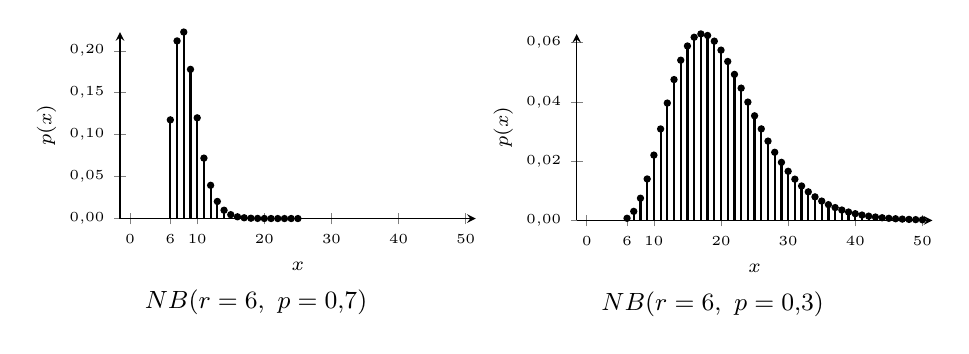
\begin{tikzpicture}
\begin{axis}[loi, xmin=0, xtick={0,6,10,20,30,40,50}, xmax=50, name=g]
  \addplot[baton] coordinates {(6,0.11765) (7,0.21177) (8,0.22236) (9,0.17789) (10,0.12007) (11,0.07204) (12,0.03962) (13,0.02038) (14,0.00993) (15,0.00464) (16,0.00209) (17,0.00091) (18,0.00039) (19,0.00016) (20,0.00007) (21,0.00003) (22,0.00001) (23,0.00000) (24,0.00000) (25,0.00000)};
\end{axis}
\node[anchor=north, font=\small] at (g.outer south) {$\text{NB}(r=6,\ p=0{,}7)$};
\begin{axis}[loi, xmin=0, xtick={0,6,10,20,30,40,50}, xmax=50, name=d, at={([xshift=0.9cm]g.outer east)}, anchor=outer west]
  \addplot[baton] coordinates {(6,0.00073) (7,0.00306) (8,0.00750) (9,0.01400) (10,0.02205) (11,0.03088) (12,0.03962) (13,0.04755) (14,0.05409) (15,0.05889) (16,0.06184) (17,0.06296) (18,0.06244) (19,0.06052) (20,0.05749) (21,0.05366) (22,0.04930) (23,0.04466) (24,0.03995) (25,0.03532) (26,0.03090) (27,0.02678) (28,0.02301) (29,0.01961) (30,0.01659) (31,0.01393) (32,0.01163) (33,0.00965) (34,0.00796) (35,0.00653) (36,0.00533) (37,0.00434) (38,0.00351) (39,0.00283) (40,0.00227) (41,0.00182) (42,0.00145) (43,0.00115) (44,0.00091) (45,0.00072) (46,0.00057) (47,0.00045) (48,0.00035) (49,0.00027) (50,0.00021)};
\end{axis}
\node[anchor=north, font=\small] at (d.outer south) {$\text{NB}(r=6,\ p=0{,}3)$};
\end{tikzpicture}
\end{center}

\medskip
{\small
Dans tous les cas :
\begin{itemize}
\item les valeurs possibles sont les entiers supérieurs ou égaux à $r$ $(r,r+1,\ldots)$;
\item plus $p$ est petit, plus les valeurs probables sont grandes;
\item plus $r$ est grand, plus les valeurs probables sont grandes.
\end{itemize}
}

\end{frame}

\begin{frame}[t]{Loi binomiale négative : espérance et variance}

\alerter{Si $X \sim \mbox{NB}(r,p)$, on peut écrire
$$ X = Y_1 + \cdots + Y_r,$$
où les $Y_i$ sont indépendantes et $Y_i \sim \mbox{Géométrique}(p)$ pour tout $i$.}
\vspace{0.1 in}

Donc,
$$E(X) = \frac{r}{p}$$
et
$$V(X) = r\,\frac{1-p}{p^2}.$$

\end{frame}

\section{Loi de Poisson}

\begin{frame}[t]{Loi de Poisson : d'où vient-elle?}

{\small
On obtient habituellement une loi de Poisson dans l'une des
deux situations suivantes :
\begin{itemize}
\item {\bf Loi des événements rares :} soit $X$ une
v.a. binomiale où $n$ est très, très grand et $p$
très, très petit. Soit $\mu$ la limite de $np$ quand
$n\to\infty$ et $p\to0$. On peut montrer qu'à la limite,
on obtient
$$p(x)=\left\{\begin{array}{ll}
\frac{\mu^x e^{-\mu}}{x!}, & x=0,1,2,\ldots,\\
0, & \text{sinon}.\end{array}\right.$$
\item {\bf Nombre d'événements dans un intervalle de temps fixé
({\it processus de Poisson}) :}
sous certaines conditions, si on observe en moyenne $\lambda$
événements par unité de temps (ou d'espace), alors le
nombre d'événements $X$ dans $t$ unités de temps (ou d'espace) suit
une loi de Poisson de moyenne $\mu=\lambda t$. \\
(On y reviendra au module 4.)
\end{itemize}
}
\end{frame}

\begin{frame}{Loi de Poisson : fonction de probabilité}
Si $X\sim \text{Poisson}(\mu)$, alors
$$p(x)=\left\{\begin{array}{ll}
\frac{\mu^x e^{-\mu}}{x!}, & x=0,1,2,\ldots,\\
0, & \text{sinon},\end{array}\right.$$

\vspace{0.2in}
et
$$E(X)=\mu \qquad\qquad V(X)=\mu.$$

\vspace{0.2in}
Voir les preuves à la page 125 du manuel.
\end{frame}

\begin{frame}{Loi de Poisson : allure}

\begin{center}
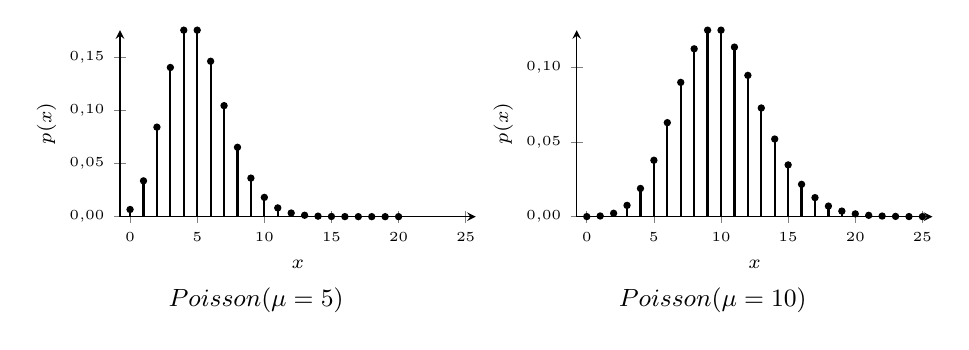
\begin{tikzpicture}
\begin{axis}[loi, xtick={0,5,...,25}, xmax=25, name=g]
  \addplot[baton] coordinates {(0,0.00674) (1,0.03369) (2,0.08422) (3,0.14037) (4,0.17547) (5,0.17547) (6,0.14622) (7,0.10444) (8,0.06528) (9,0.03627) (10,0.01813) (11,0.00824) (12,0.00343) (13,0.00132) (14,0.00047) (15,0.00016) (16,0.00005) (17,0.00001) (18,0.00000) (19,0.00000) (20,0.00000)};
\end{axis}
\node[anchor=north, font=\small] at (g.outer south) {$\text{Poisson}(\mu=5)$};
\begin{axis}[loi, xtick={0,5,...,25}, xmax=25, name=d, at={([xshift=0.9cm]g.outer east)}, anchor=outer west]
  \addplot[baton] coordinates {(0,0.00005) (1,0.00045) (2,0.00227) (3,0.00757) (4,0.01892) (5,0.03783) (6,0.06306) (7,0.09008) (8,0.11260) (9,0.12511) (10,0.12511) (11,0.11374) (12,0.09478) (13,0.07291) (14,0.05208) (15,0.03472) (16,0.02170) (17,0.01276) (18,0.00709) (19,0.00373) (20,0.00187) (21,0.00089) (22,0.00040) (23,0.00018) (24,0.00007) (25,0.00003)};
\end{axis}
\node[anchor=north, font=\small] at (d.outer south) {$\text{Poisson}(\mu=10)$};
\end{tikzpicture}
\end{center}

\medskip
{\small
Dans tous les cas :
\begin{itemize}
\item les valeurs possibles sont tous les entiers non négatifs $(0,1,2,\ldots)$;
\item les valeurs les plus probables sont concentrées autour de l'espérance.
\end{itemize}
}

\end{frame}

\begin{frame}{Loi de Poisson : deux propriétés importantes}

\textbf{Additivité :}\\
Si $X_1,\ldots,X_n$ sont des v.a. indépendantes avec $X_i\sim \text{Poisson}(\mu_i)$ et
$Y=X_1+\cdots+X_n$, alors

$$Y\sim \mbox{Poisson}(\mu_1+\cdots+\mu_n).$$


\vspace{0.1in}
\textbf{Approximation de la binomiale :}\\
Lorsque $n$ est grand et $p$ est petit (par exemple $n\ge 20$ et $p\le 0{,}05$), on peut approximer la loi Binomiale$(n,p)$ par une loi Poisson$(\mu=np)$.

\end{frame}

\section{Quelques exemples}

\begin{frame}[t,label=exconn]{Connexions à un serveur}

{\small
Un programme tente de se connecter à un serveur surchargé. Chaque tentative réussit avec probabilité 1/3, indépendamment des autres.
Quelle est la probabilité qu'il faille 4, 5 ou 6 tentatives pour établir la connexion?
}

\lienreponse{rep-ex}
\end{frame}


\begin{frame}[t]{Connexions à un serveur (suite)}

{\small
Combien de tentatives faut-il en moyenne pour établir la connexion?
}

\vspace{1in}
{\small
Combien de tentatives faut-il en moyenne pour établir 5 connexions?
}
\lienreponse{rep-ex}
\end{frame}


\begin{frame}[t]{Connexions à un serveur (suite)}

{\small
Quelle est la probabilité qu'il faille plus de 6 tentatives pour établir 5 connexions?
}

\lienreponse{rep-ex}
\end{frame}


\begin{frame}[t,label=exexamen]{Examen à choix multiples}

{\small Un examen compte 20 questions à choix multiples, avec 5 choix
de réponse par question. Si on répond complètement au hasard aux 20 questions,
et qu'une bonne réponse vaut 10 points et une mauvaise réponse $-2$ points,
quel est notre score attendu à cet examen?
}
\lienreponse{rep-ex}
\end{frame}

\begin{frame}[t,label=exbogues]{Des bogues dans le code}

{\small
Le nombre de bogues dans un logiciel suit une loi de Poisson de moyenne
1 bogue par 10~000 lignes de code. Quelle est la probabilité qu'un module
de 20~000 lignes contienne au moins un bogue?

\vspace{1.5in}
Quel est le nombre moyen de bogues dans de tels modules?
}
\lienreponse{rep-ex}
\end{frame}


\begin{frame}[t,label=exrevenus]{Calcul de revenus}

{\small
Une firme d'informaticiens est engagée pour concevoir un logiciel de prise de rendez-vous. Elle sera payée 25~000~\$ pour ce travail, plus une prime de 5~000~\$ si le logiciel est terminé à la date prévue. Quelles sont la moyenne et la variance des revenus de cette firme pour ce contrat si la probabilité de terminer à temps est de 20~\%?
}
\lienreponse{rep-ex}
\end{frame}

\begin{frame}[t,label=exbits]{Bits aléatoires}

{\small
Un générateur produit 10 bits aléatoires indépendants; chacun vaut 1 avec probabilité 1/2. Calculez
\begin{enumerate}
 \item[(i)] l'espérance et la variance du nombre de 1 obtenus;
 \item[(ii)] la probabilité d'obtenir exactement deux 1;
 \item[(iii)] la probabilité d'obtenir au moins deux 1.
\end{enumerate}
}
\lienreponse{rep-ex}
\end{frame}


\begin{frame}[t,label=exentrevues]{Des entrevues}

{\small
 Une entreprise doit faire passer des entrevues jusqu'à l'embauche de
 2 nouveaux développeurs. Chaque entrevue mène à une embauche avec probabilité 25~\%,
 et les décisions prises aux différentes entrevues sont indépendantes. Une entrevue
 qui mène à une embauche coûte 500~\$ et une entrevue qui n'y mène pas coûte 100~\$.
 Quels sont l'espérance et l'écart-type du coût total des entrevues?
}
\lienreponse{rep-ex}
\end{frame}

\section{Compléments}

\begin{frame}{Loi géométrique : vérification}

Vérifiez que la fonction de probabilité de la loi géométrique,
$p(x)=(1-p)^{x-1}p$ pour $x=1,2,\ldots$, est bien une fonction de probabilité.
\vspace{5cm}

\end{frame}

\section{Réponses des exemples}

\begin{frame}[t,label=rep-ex]{Réponses des exemples}
\footnotesize
\begin{itemize}
\item \retour{exconn}{Connexions à un serveur} : $P(X\in\{4,5,6\})=152/729\approx0{,}2085$~;
(suite) en moyenne $E(X)=1/p=3$ tentatives pour une connexion et $E(X)=r/p=15$ tentatives pour 5 connexions~;
(suite) $P(X>6 \mbox{ pour 5 connexions})=716/729\approx0{,}9822$.
\item \retour{exexamen}{Examen à choix multiples} : score attendu $=20\times(10\times0{,}2-2\times0{,}8)=8$ points.
\item \retour{exbogues}{Des bogues dans le code} : $\mu=2$ bogues pour 20~000 lignes~;
$P(X\ge1)=1-e^{-2}\approx0{,}8647$~; moyenne $=\mu=2$ bogues.
\item \retour{exrevenus}{Calcul de revenus} : $E(Y)=26~000~\$$~; $V(Y)=4~000~000~\$^2$.
\item \retour{exbits}{Bits aléatoires} : (i) $E(X)=5$, $V(X)=2{,}5$~;
(ii) $P(X=2)=45/1024\approx0{,}0439$~; (iii) $P(X\ge2)\approx0{,}9893$.
\item \retour{exentrevues}{Des entrevues} : $E(Y)=1~600~\$$~; $V(Y)=240~000~\$^2$ ($\sigma_Y\approx489{,}9~\$$).
\end{itemize}

\end{frame}

\begin{frame}{Bibliographie}
 	Ce document est rédigé avec Beamer ainsi qu'une classe .cls fournie par Jérôme Soucy. Les diapositives sont adaptées des diapositives créées par Anne-Sophie Charest
 pour le cours STT-1000.
 	\printbibliography
 	\vfill
 	\footnotesize Pour signaler une erreur dans ce document, veuillez écrire à l'adresse :~\href{mailto:julien.miron@mat.ulaval.ca}{julien.miron@mat.ulaval.ca}.
 \end{frame}

\end{document}
